\section{Interface Design Description}
Dit hoofstuk behandeld in detail alle interfaces en communicatie de het systeem
en daarmee subsystemen met elkaar hebben.

\subsection{Interface design}
\begin{center}
\hspace*{-3.5cm}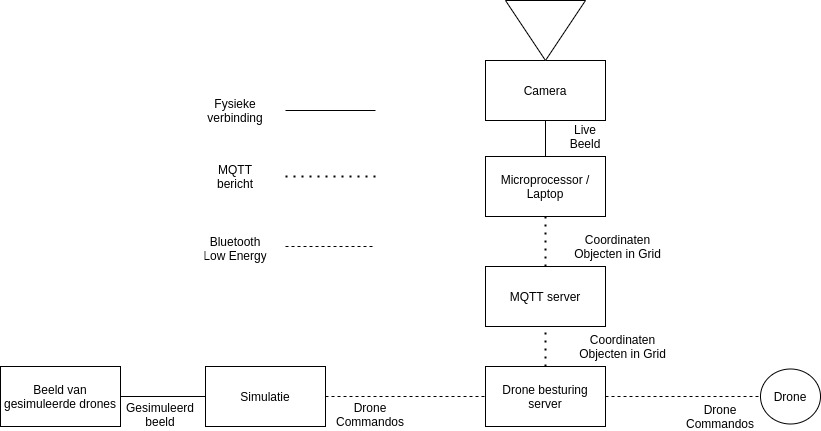
\includegraphics[width=1.6\textwidth]{../IMAGES/IDD.jpg}
\end{center}
	Zoals in de afbeelding te zien is, hangt het gehele systeem samen met elkaar en zijn afhankelijk van elkaar, ondanks dat er verschillende lagen tussen de onderdelen zijn. Voor communicatie tussen verschillende apparaten wordt MQTT gebruikt, terwijl voor verschillende onderdelen van dezelfde apparaat er gebruik gemaakt wordt van een eigen communicatie methode. Zo is dat tussen de camera met de laptop een seriele kabel en tussen de simulatie en het beeldscherm een GPU om de gesimuleerde drones af te kunnen beelden. Tussen de server en de drone wordt er gebruik gemaakt van een draadloze manier van communiceren, namelijk bluetooth. Specifiek bluetooth low energy, gezien de drones een kleine batterij heeft en dus zo veel mogelijk stroom moet besparen. Op deze manier hangt het systeem samen. Er is dus geen gebruiker binnen het systeem, maar wel end-points. Zo zijn de camera, drone en gesimuleerde drones endpoints. Gebruikers buiten het systeem nemen waar wat er gebeurt met deze drones en kunnen op basis daarvan conclusies trekken over het gedrag van bijen. De camera wordt end-point genoemd, maar is eigenlijk het begin van het gehele systeem. Deze stuurt namelijk een beeld op van het veld en de huidige objecten binnen het veld, zoals drones, eten en de bijenkorf. Dit beeld wordt verwerkt op de microprocessor of laptop, en stuurt als resultaat een MQTT bericht op met de locaties van ieder object. De server voor het aansturen van de drones is geabboneerd op dezelfde kanaal en kan de berichten uitlezen. Wat de drones uiteindelijk moeten gaan doen wordt dan naar de simulatie en de fysieke drones gestuurd. Op deze manier voeren de drones hun taak uit.

\subsection{Interface identification and diagrams}
